\part{HPC Facilities}
\begin{frame}
\partpage
\end{frame}

\section{CSD3}
\begin{frame}{CSD3 - University of Cambridge}
\begin{itemize}
\item{Cambridge Service for Data Driven Discovery}
\pause
\medskip
\item{\alert{Peta4 --- Intel CPU cluster}}
\pause
\item{\alert{Wilkes2 --- NVIDIA GPU cluster}}
\pause
\medskip
\item{Hadoop-based data analytic platform}
\item{Burst buffer}
\item{Industry users through CORE.}
\end{itemize}
\end{frame}

\section{Peta4-Skylake}
\begin{frame}{Peta4-Skylake}
\begin{itemize}
\item{Each compute node:}
\begin{itemize}
\item[$\ast$]{\only<1>{2x16 cores, Intel Skylake 2.6 GHz}\only<2->{{\color{red}32 CPUs}}}
\item[$\ast$]{\only<1>{$192\,\text{GB}$ or $384\,\text{GB}$ RAM}\only<2->{{\color{red}$6\,\text{GB}$ or $12\,\text{GB}$ per CPU}}}
\item[$\ast$]{\only<1>{$100\,\text{Gb/sec}$ Omni-Path}\only<2->{\color{red}$10\,\text{GB/sec}$ (for MPI and storage)}}
\end{itemize}
\item{768 compute nodes}
\item{8 login nodes (\alert{login-cpu.hpc.cam.ac.uk})}
\end{itemize}
\end{frame}

%\section{Coprocessors --- GPUs etc}
%\begin{frame}{Coprocessors --- GPUs etc}
%  \begin{itemize}
%  \item{CPUs are \alert{general purpose}}
%    \pause
%  \item{Some types of parallel workload fit \alert{vector} processing well:}
%    \begin{itemize}
%    \item{Single Instruction, Multiple Data (SIMD)}
%    \item{\emph{Think pixels on a screen}}\pause
%    \item{GPUs specialise in this type of work}\pause
%      \item{Also competitor many-core architectures such as the Intel Phi}
%    \end{itemize}
%\end{itemize}
%\end{frame}

\section{Wilkes2-GPU}
\begin{frame}{Wilkes2-GPU}
\begin{itemize}
\item{Each compute node:}
\begin{itemize}
\item[$\ast$]{\only<1>{$4\times\text{NVIDIA P100 GPU}$}\only<2->{\color<2->{red}4 GPUs}}
\item[$\ast$]{\only<1>{1x12 cores, Intel Broadwell 2.2 GHz}\only<2->{{\color{red}12 CPUs}}}
\item[$\ast$]{\only<1>{$96\,\text{GB}$ RAM}\only<2->{{\color{red}$96\,\text{GB}$ RAM}}}
\item[$\ast$]{\only<1>{$100\,\text{Gb/sec}$ (4X EDR) Infiniband.}\only<2->{\color{red}$10\,\text{GB/sec}$ (for MPI and storage)}}
\end{itemize}
\item{90 compute nodes.}
\item{8 login nodes (\alert{login-gpu.hpc.cam.ac.uk}).}
\end{itemize}
\end{frame}

\section{Peta4-KNL}
\begin{frame}{Peta4-KNL (Intel Phi)}
\begin{itemize}
\item{Each compute node:}
\begin{itemize}
\item[$\ast$]{\only<1>{64 cores, Intel Phi 7210}\only<2->{{\color{red}256 CPUs}}}
\item[$\ast$]{\only<1>{$96\,\text{GB}$ RAM}\only<2->{{\color{red}$96\,\text{GB}$ RAM}}}
\item[$\ast$]{\only<1>{$100\,\text{Gb/sec}$ Omni-Path}\only<2->{\color{red}$10\,\text{GB/sec}$ (for MPI and storage)}}
\end{itemize}
\item{342 compute nodes}
\item{Shared login nodes with Peta4-Skylake}
\end{itemize}
\end{frame}


%\begin{frame}{HPCS Production Cluster Schematic}
%\centerline{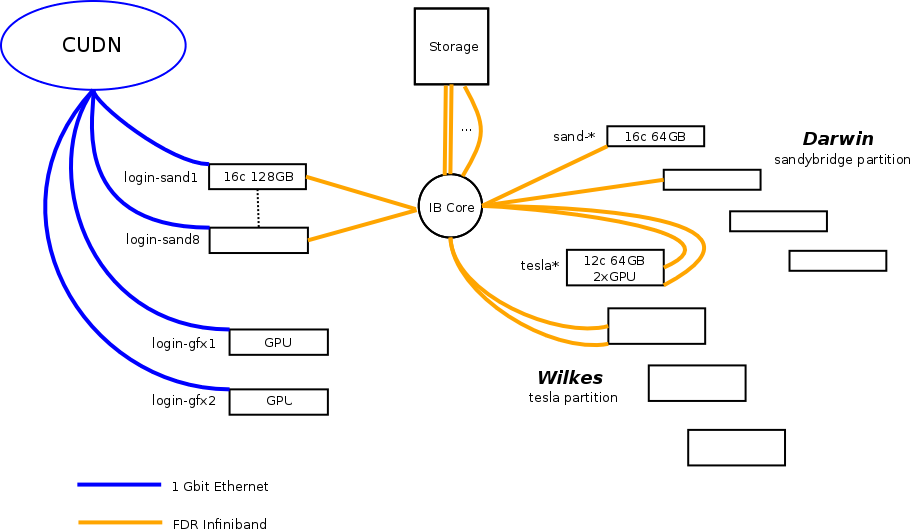
\includegraphics[width=0.95\textwidth]{imgs/cluster.png}}%
%\end{frame}

\section{Storage}
\begin{frame}{HPCS: Storage}
\begin{itemize}
\item{Multi-petabytes split across multiple filesystems with tape.}
\item{Lustre cluster filesystem:}
\begin{itemize}
\item[$\ast$]{Multiple RAID6 back-end disk volumes.}
\item[$\ast$]{Multiple object storage servers.}
\item[$\ast$]{Single metadata server.}
\item[$\ast$]{Tape-backed HSM on newest filesystems.}
\pause
\item[$\ast$]{\alert{$4\,\text{GB/sec}$ overall read or write.}}
\pause
\item[$\ast$]{\alert{Prefers big read/writes over small.}}
\end{itemize}
\pause
\item{\alert{For active HPC work only.}}
\end{itemize}
\end{frame}

\section{Obtaining an Account and Support}
\begin{frame}{Obtaining an Account and Support}
\begin{itemize}
\item{To apply for an account, complete our online form:}
\item \small {\url{https://www.csd3.cam.ac.uk/services/applying-for-resources}}
\pause
\item{For support enquiries please email our Service Desk:}
\item{\alert{support@hpc.cam.ac.uk}}
\end{itemize}
\end{frame}